\documentclass[border=15pt]{standalone}
\usepackage{tikz}
\usetikzlibrary{arrows.meta, positioning, calc}

\begin{document}

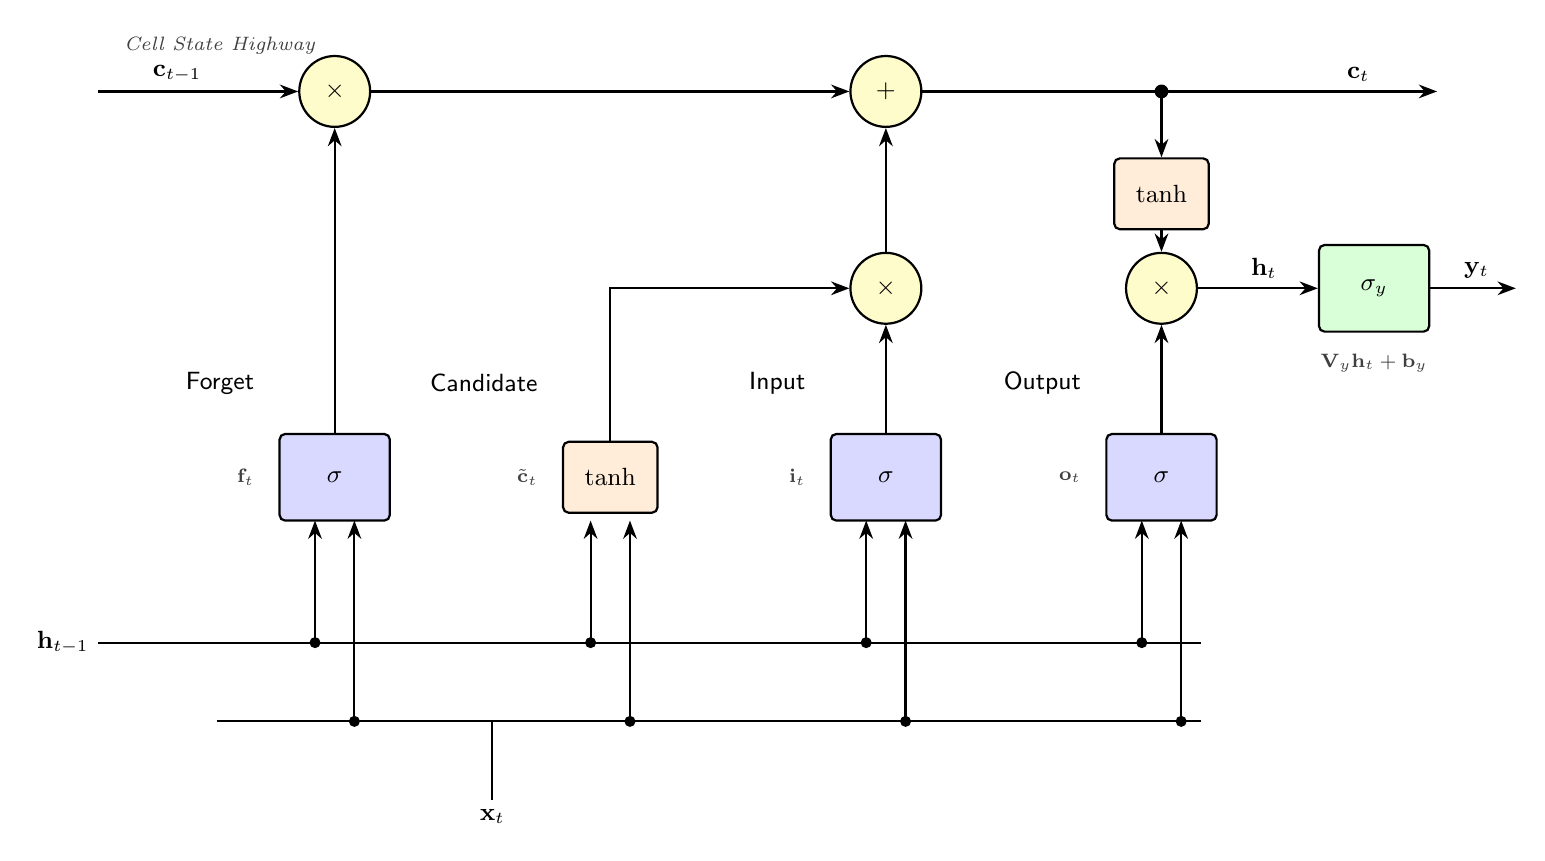
\begin{tikzpicture}[
    >=Stealth,
    gate/.style={
        rectangle, draw, thick, minimum width=1.4cm, minimum height=1.1cm,
        fill=blue!15, font=\small\bfseries, rounded corners=2pt
    },
    op/.style={
        circle, draw, thick, minimum size=0.9cm, fill=yellow!20,
        font=\small\bfseries, inner sep=0pt
    },
    act/.style={
        rectangle, draw, thick, minimum width=1.2cm, minimum height=0.9cm,
        fill=orange!15, font=\small, rounded corners=2pt
    },
    outblock/.style={
        rectangle, draw, thick, minimum width=1.4cm, minimum height=1.1cm,
        fill=green!15, font=\small\bfseries, rounded corners=2pt
    },
    arr/.style={draw, thick, ->},
    lbl/.style={font=\small},
    eqlbl/.style={font=\scriptsize, text=gray!50!black},
    gatelbl/.style={font=\small\sffamily, anchor=east},
]

% ================================================================
%  COLUMN POSITIONS (well separated)
% ================================================================
\def\colF{2}       % forget gate
\def\colC{5.5}     % candidate
\def\colI{9}       % input gate
\def\colO{12.5}    % output gate

% ROW POSITIONS
\def\rowHighway{8.5}     % cell state highway
\def\rowTanhC{7.2}       % tanh of cell state (output path)
\def\rowMulO{6.0}        % output multiply
\def\rowMulI{6.0}        % input multiply (same row as output multiply)
\def\rowGateLabel{4.8}   % gate label row
\def\rowGate{3.6}        % gate row
\def\rowBusH{1.5}        % h_{t-1} bus
\def\rowBusX{0.5}        % x_t bus
\def\rowOut{0.5}         % output projection y

% ================================================================
%  CELL STATE HIGHWAY
% ================================================================
\node[op] (mul_f) at (\colF, \rowHighway) {$\times$};
\node[op] (add_c) at (\colI, \rowHighway) {$+$};

% c_{t-1} arrow
\draw[arr] (-1, \rowHighway) -- (mul_f.west);
\node[lbl, above] at (0, \rowHighway) {$\mathbf{c}_{t-1}$};

% forget-multiply -> add
\draw[arr] (mul_f.east) -- (add_c.west);

% add -> c_t out
\draw[arr] (add_c.east) -- (16, \rowHighway);
\node[lbl, above] at (15, \rowHighway) {$\mathbf{c}_{t}$};

% branch point for output gate tanh
\fill (\colO, \rowHighway) circle (2.5pt);

% "Cell State Highway" label
\node[eqlbl, anchor=south west] at (-0.8, \rowHighway+0.35)
    {\textit{Cell State Highway}};

% ================================================================
%  FOUR GATE/CANDIDATE BLOCKS
% ================================================================
\node[gate] (fg) at (\colF, \rowGate) {$\sigma$};
\node[act]  (cand) at (\colC, \rowGate) {$\tanh$};
\node[gate] (ig) at (\colI, \rowGate) {$\sigma$};
\node[gate] (og) at (\colO, \rowGate) {$\sigma$};

% Labels to the LEFT of each block (anchor=east so text ends before the block)
\node[gatelbl] at (\colF-0.9, \rowGateLabel) {Forget};
\node[gatelbl] at (\colC-0.8, \rowGateLabel) {Candidate};
\node[gatelbl] at (\colI-0.9, \rowGateLabel) {Input};
\node[gatelbl] at (\colO-0.9, \rowGateLabel) {Output};

% ================================================================
%  FORGET GATE -> CELL STATE
% ================================================================
\draw[arr] (fg.north) -- (mul_f.south);

% ================================================================
%  INPUT GATE + CANDIDATE -> CELL STATE
% ================================================================
\node[op] (mul_i) at (\colI, \rowMulI) {$\times$};

% Input gate -> multiply
\draw[arr] (ig.north) -- (mul_i.south);

% Multiply -> add on highway
\draw[arr] (mul_i.north) -- (add_c.south);

% Candidate -> multiply (route up then right)
\draw[arr] (cand.north) -- (\colC, \rowMulI) -- (mul_i.west);

% ================================================================
%  OUTPUT GATE -> h_t
% ================================================================
% tanh of cell state (more space above multiply)
\node[act] (tanh_c) at (\colO, \rowTanhC) {$\tanh$};
\draw[arr] (\colO, \rowHighway) -- (tanh_c.north);

% Output multiply node (well below tanh)
\node[op] (mul_o) at (\colO, \rowMulO) {$\times$};
\draw[arr] (tanh_c.south) -- (mul_o.north);
\draw[arr] (og.north) -- (mul_o.south);

% h_t exits to the right, inline with output projection
\node[outblock] (out_proj) at (15.2, \rowMulO) {$\sigma_y$};
\draw[arr] (mul_o.east) -- (out_proj.west);
\node[lbl, above] at (13.8, \rowMulO) {$\mathbf{h}_t$};
\draw[arr] (out_proj.east) -- (17, \rowMulO);
\node[lbl, above] at (16.5, \rowMulO) {$\mathbf{y}_t$};
\node[eqlbl, below=4pt of out_proj]
    {$\mathbf{V}_y\mathbf{h}_t + \mathbf{b}_y$};

% ================================================================
%  INPUT BUSES
% ================================================================

% ---- h_{t-1} horizontal bus ----
\draw[thick] (-1, \rowBusH) -- (\colO+0.5, \rowBusH);
\node[lbl, left] at (-1, \rowBusH) {$\mathbf{h}_{t-1}$};

% ---- x_t horizontal bus ----
\draw[thick] (0.5, \rowBusX) -- (\colO+0.5, \rowBusX);

% x_t entry from below
\node[lbl, below] at (4, -0.5) {$\mathbf{x}_t$};
\draw[thick] (4, -0.5) -- (4, \rowBusX);

% ---- Risers from h_{t-1} bus (left arrow of each gate pair) ----
\foreach \col in {\colF, \colC, \colI, \colO} {
    \draw[arr] (\col-0.25, \rowBusH) -- (\col-0.25, \rowGate-0.55);
    \fill (\col-0.25, \rowBusH) circle (2pt);
}

% ---- Risers from x_t bus (right arrow of each gate pair) ----
\foreach \col in {\colF, \colC, \colI, \colO} {
    \draw[arr] (\col+0.25, \rowBusX) -- (\col+0.25, \rowGate-0.55);
    \fill (\col+0.25, \rowBusX) circle (2pt);
}

% ================================================================
%  VARIABLE LABELS (to the left of each gate, clear of risers)
% ================================================================
\node[eqlbl, anchor=east] at (\colF-0.9, \rowGate) {$\mathbf{f}_t$};
\node[eqlbl, anchor=east] at (\colC-0.8, \rowGate) {$\tilde{\mathbf{c}}_t$};
\node[eqlbl, anchor=east] at (\colI-0.9, \rowGate) {$\mathbf{i}_t$};
\node[eqlbl, anchor=east] at (\colO-0.9, \rowGate) {$\mathbf{o}_t$};

\end{tikzpicture}

\end{document}
